\chapter{Software}
\par Este componente de software tendrá el propósito de asistir al fabricante de cerveza en las tareas de monitoreo, planificación y visualización de datos históricos de experimentos de maceración.

\par En los siguientes incisos, serán descriptas las consideraciones tomadas para la elección de una plataforma sobre la cual se desarrollará la aplicación de Software.

\section{Análisis de alternativas}
    \subsection{Tecnologías}
        \par A continuación se presenta una breve reseña de las plataformas actualmente más relevantes para dispositivos móviles.
        
        \subsubsection{Android}
            \par Android es un sistema operativo, el cual fue inicialmente desarrollado por Android Inc., empresa que Google respaldó económicamente y más tarde, en 2005, compró. Fue diseñado principalmente para dispositivos móviles con pantalla táctil desarrollados por Google o por terceros, como teléfonos inteligentes, tabletas y también, relojes inteligentes, televisores y automóviles. 
            
            \par Android es un sistema operativo basado en el núcleo Linux.
            
        \subsubsection{iOS}
            \par iOS es un sistema operativo móvil de la multinacional Apple Inc. Originalmente desarrollado para el iPhone (iPhone OS), después utilizado en dispositivos como el iPod touch y el iPad. No permite la instalación de iOS en hardware de terceros.
            
            \par iOS se deriva de macOS, que a su vez está basado en Darwin BSD, y por lo tanto es un sistema operativo Tipo Unix.
            
  
            
            
    \subsection{Comparación}
        \par El desarrollo será realizado para una plataforma móvil, de las cuales se tendrán en cuenta las siguientes consideraciones: cantidad de usuarios que la utilicen; tamaño de la comunidad a disposición para dar soporte; disponibilidad de mejores herramientas y utilidades para el desarrollo de aplicaciones.
        
        \par A continuación, se presenta una tabla comparativa en la cual se abordan aspectos de interés para la elección y un análisis concluyente.
        
        \begin{table}[h]
            \centering
            \begin{tabularx}{\textwidth}{|X|X|X|}
                 \hline
                 \multicolumn{3}{|c|}{Tabla comparativa de tecnologías de software}\\
                 \hline
                 Criterios de comparación & Android & iOS \\
                 \hline
                 \hline
                 
                 Porcentaje Mercado (Arg) & 75\% & 19\%  \\
                 \hline
                 
                 Porcentaje Mercado Internacional & 85\% & 14,7\% \\
                 \hline
                 
                 Comunidad de desarrolladores & Muy grande & Amplia pero acorde al número de usuarios\\
                 \hline
                 
                  Entornos desarrollo Propia & Android Studio & Xcode\\
                 \hline
                 
                 Lenguaje de desarrollo & Java, C, C++ y Kotlin & Swift, C, C++ y objective-C\\
                 \hline
                 
                 Familia del SO & Linux & Unix - BSD\\
                 \hline
                 
                 Complejidad de desarrollo & Muy diversa variedad de dispositivos y de versiones del SO & Variedad reducida de dispositivos, versiones de SO comunes a la mayoría\\
                 \hline
                 
                 Entorno & Open Source & Entorno cerrado \\
                 \hline
                 
                 Requerimientos para publicación de aplicación & Ninguna & Debe cumplir requisitos de Apple\\
                 \hline
                 
            \end{tabularx}
            \caption{Comparación de plataformas móviles}
            \label{tab:ComparacionPlataformasMoviles}
        \end{table}

    
    \subsection{Elección}
    \par
    La elección fue realizada a partir de los criterios antes mencionados aplicados sobre la tabla comparativa.
    \par
    Se decidió desarrollar la aplicación para la plataforma \textbf{Android}, considerado, el porcentaje de uso en Argentina, el tamaño de la comunidad de desarrolladores, la gran disponibilidad de herramientas y la sencillez relativa en cuanto a requerimientos para la publicación de aplicaciones.
    
    \par Para el desarrollo se empleó el lenguaje Java (JDK 1.7 o Java 7) sobre el entorno de desarrollo integrado (IDE) oficial de Google, AndroidStudio. La versión de sistema operativo mínima para la que se desarrolló es \textit{Nougat 7.0}, lanzada en agosto de 2016, la cual utiliza la plataforma de desarrollo (Android SDK plataform \footnote{\url{https://developer.android.com/studio/releases/platforms}}) API nivel 24.

    
    
\section{Diseño}
    \subsection{Diseño de la interfaz de usuario}
        \par Las figuras \ref{fig:MockUpMainActivity}, \ref{fig:MockUpPlanningActivity}, \ref{fig:MockUpExperimentActivity}, \ref{fig:MockUpInfoMash}, \ref{fig:MockUpCurrentExperienceFragment}, \ref{fig:MockUpStageFragment}, \ref{fig:MockUpGeneralFragment}, \ref{fig:MockUpExperimentFragment} y \ref{fig:MockUpDetailExperimentActivity} ubicadas en el Anexo, diagraman y describen el diseño y las funcionalidades de la interfaz de usuario (UI) bosquejadas para la aplicación móvil.

    \subsection{Base de Datos}
        \par En el siguiente diagrama (Figura \ref{fig:DiagramaBdApp}) se esquematiza la base de datos a alojar en la aplicación. En el diagrama se pueden distinguir las tablas a utilizar para la abstracción de la aplicación y el conjunto de relaciones establecidas entre ellas.
        
        \begin{figure}[h]
            \centering
            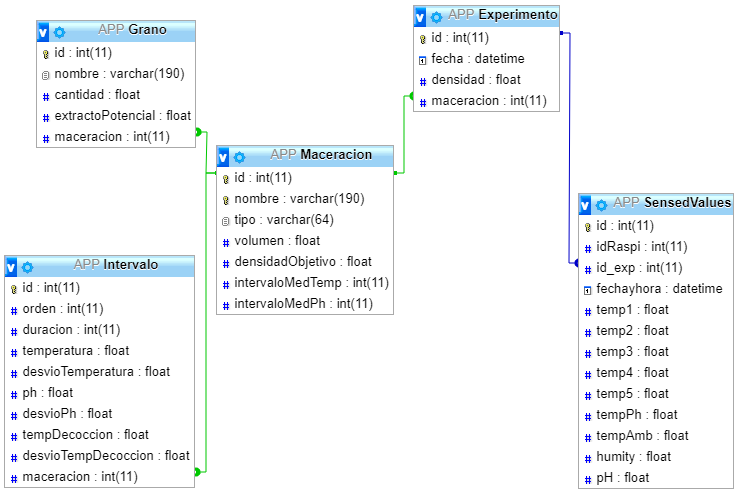
\includegraphics[scale=0.8]{DiagramaBaseDeDatosAPP.jpg}
            \caption{Diagrama de Base de Datos de la aplicación}
            \label{fig:DiagramaBdApp}
        \end{figure}

\section{Implementación}
    \par En esta sección, se realizará en primer lugar una breve introducción al desarrollo Android de manera de construir una base de conocimientos del tema. Luego, para cada pantalla implementada se realizará una descripción estética y funcional junto a un detalle de su implementación.
    
    \subsection{Breve introducción al desarrollo en Android}
    
    \par Las aplicaciones en Androdid son desarrolladas siguiendo el patrón de arquitectura de desarrollo MVP (Modelo-Vista-Presentador). Este patrón separa las lógicas de datos y negocios (modelo y presentador respectivamente) de la interfaz gráfica (Vista). En este contexto, la lógica es llevada a cabo por elementos denominados \textit{Activities} y Adaptadores (\textit{Adapters}) y componentes de interfaz gráfica denominados Vistas(\textit{Views}).
    
    \par En cada clase \textit{Activity} es definida la lógica de funcionamiento de la aplicación y el manejo de una pantalla relacionada a esta con la que el usuario finalmente interactúa. Entre las funcionalidades implementadas dentro de un \textit{Activity} pueden mencionarse principalmente: gestión de widgets\footnote{Elementos gráficos preestablecidos que implementan funcionalidades, como menús desplegables, botones, relojes, etc.} desplegados en la pantalla; lógica o dinámica de funcionamiento; manejo de información ingresada y desplegada en pantalla; llamadas a librerías externas de interacción con bases de datos, APIs o incluso otros \textit{Activities}.
    
    % ------ Ver si es necesario hablar de ciclo de vida del activity.
    \subsubsection{Interfaz gráfica}
    
    \par Una estructura de pantalla básica esta compuesta por un \textit{Actionbar} y un cuerpo (Véase Figura \ref{fig:emptyActivity}). El primero se ubica en la parte superior  y contiene el título de la pantalla o aplicación y soporta el agregado de un \textit{OptionsMenu} (compuesto por botones y/o un menú desplegable). En el segundo se ubicará el contenedor de Vistas (layout) y el contenido gráfico-funcional a ser definido para esta pantalla.
    
    \begin{figure}
        \centering
        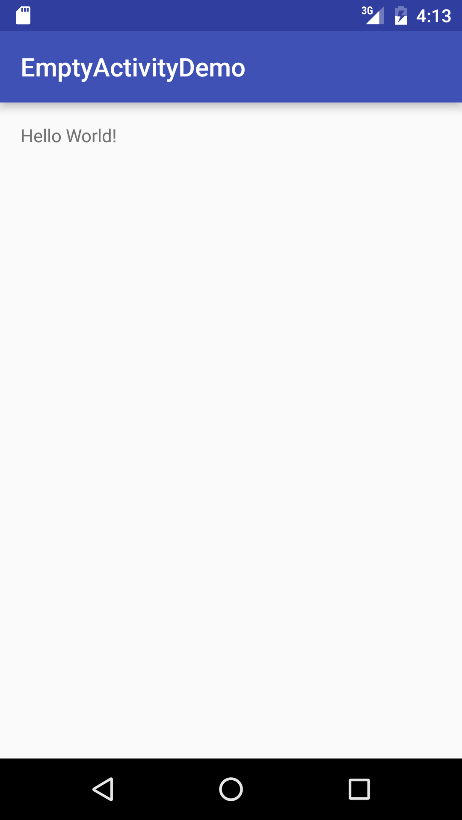
\includegraphics[scale=0.5]{software/EmptyActivity.jpg}
        \caption{\textit{EmptyActivity} - Pantalla básica en Android: ActionBar(Azul con texto EmptyActivityDemo) y Cuerpo (Blanco con texto Hello World!)}
        \label{fig:emptyActivity}
    \end{figure}
    
    \par Android organiza los componentes visuales de una pantalla mediante archivos XML. En estos puede ser definida la estructura básica de una pantalla (posiciones, margenes, etc.) y ser agregados layouts o widgets. De entre los componentes tipo widget pueden ser mencionados los botones estáticos (\textit{Button}) o flotantes (\textit{FloatingActionButton}), menús desplegables (\textit{Spinner}), campos para inserción y presentación de texto (\textit{EditText y TextView respectivamente}), entre otros.
    
    %Le clavo itemize?
    %\begin{minipage}[0.95\textwidth]
    \par Dentro de los layouts disponibles se encuentran:
    
    \begin{itemize}
        \item \textit{LinearLayout}, que permite definir en secuencia vertical(arriba hacia abajo)  u horizontal(izquierda a derecha) el orden en que se visualizan los componentes;
        \item \textit{RelativeLayout} que define la ubicación en pantalla del componente en referencia a otro componente ya añadido;
        
        \item \textit{FrameLayout} que define la ubicación de los componentes de manera absoluta, permitiendo la superposición de los mismos;
        
        \item \textit{ScrollView}, utilizado cuando el espacio en pantalla es menor que el contenido que se desea mostrar, ofreciendo la posibilidad de desplazar el mismo para visualizar el área de interés de este contenido;
        
        \item \textit{ListView} que generan una lista de layout anidados, utilizado cuando la cantidad de estos últimos varia dinámicamente. Para el manejo de los mismos, se utiliza un tipo de clase denominado \textit{Adapter} que gestiona la información de cada entrada de la lista y como se visualiza dentro de la misma;
        
        \item \textit{RecyclerView} posee la misma funcionalidad que el \textit{ListView} pero este no renderiza los layout que no se muestran en pantalla, como si lo hace el primero. Se utiliza cuando la cantidad de layout anidados es bastante mayor que lo que puede ser mostrado en pantalla. Donde, el requerimiento de memoria para mantener todo el conjunto de entradas podría producir una reducción del rendimiento de la aplicación;
        
        \item \textit{CardView} es un contenedor estético que usualmente presenta un panel de bordes redondeados y sombra, muy utilizado en conjunto con \textit{RecyclerView} o \textit{ListView} como layout anidado dentro los mismos.
        
    \end{itemize}

    %\end{minipage}
    
    \par Una pantalla puede incorporar, además de \textit{Views}, cuadros de diálogo (pop-up) emergentes y menús contextuales (\textit{ContextMenu}) que son invocados a través de la interacción del usuario con un \textit{View}. Para la definición del contenido visual y el comportamiento de estos diálogos se utiliza la clase \textit{AlertDialog} para una ventana tipo emergente y métodos propios del \textit{Activity} para un menú contextual. Ambos casos, se implementan dentro del \textit{Activity} encargado de gestionar esa pantalla.
    
    \par Como fue antes mencionado, la lógica funcional de una pantalla es implementada en un \textit{Activity}. Dentro de este pueden ser incluidos \textit{Fragments}, los cuales representan un comportamiento o una parte de la interfaz de usuario. Permitiendo con su uso combinado en una misma actividad crear interfaces gráficas multipanel. El manejo de las pantallas o interfaces definidas para un \textit{Fragment} se realiza de la misma forma que las pantallas definidas para un \textit{Activity}.
    
    \par Una forma de utilizar \textit{Fragments} es mediante pestañas (\textit{Tabs}). De esta manera una misma pantalla contiene un conjunto definido de cuerpos intercambiables (subpantallas). Para su manipulación por el usuario son utilizados \textit{TabLayouts} que definen el conjunto de pestañas en la pantalla junto a clases instanciadas por el Activity padre encargados de gestionar los intercambios entre las mismas (\textit{ViewPagerAdapter}).
    
    %\par En la implementación de los componentes de la interfaz gráfica (Views) pueden ser incorporados \textit{listeners} los cuales definen un comportamiento u operación a ser realizada según la forma en la que el usuario interactúe con los mismos. Ejemplos de estos últimos son el click (\textit{onClickListener}), click de larga duración (\textit{onLongClickListener}), desplazamiento vertical u horizontal (\textit{onScrollListener}), entre otros.
    
    
    \subsubsection{Librerías externas}
     \par Los \textit{Activities} dentro de su hilo de ejecución incluyen métodos o llamadas que interaccionan con librerías o clases complementarias. Se considera importante mencionar las siguientes:
     \begin{itemize}
         \item \textbf{Clases POJO} (Plain Old Java Object): Utilizadas en el modelado de las reglas de negocio, se utilizan clases complementarias que estructuran y relacionan la información requerida mediante la definición de sus atributos y métodos.
         
         \item \textbf{Persistencia}: Pueden ser utilizadas distintas librerías\footnote{https://developer.android.com/guide/topics/data/data-storage}. En el desarrollo de esta aplicación se utilizó persistencia de datos y almacenamiento de preferencias compartidas (datos de configuración). Para el primero, se decidió gestionar la base de datos SQL en Android utilizando \textit{SQLite}\footnote{SQLite, sistema de gestión de bases de datos relacional}. En su implementación, se define una clase con patrón \textit{Singleton}\footnote{Singleton, patrón de diseño que permite restringir la creación de objetos pertenecientes a una clase o el valor de un tipo a un único objeto} que define la estructura de tablas de la base de datos y en la que, adicionalmente, se pueden implementar funciones para actualizar, insertar, eliminar y consultar datos de las tablas. Para el segundo, preferencias compartidas, se utiliza \textit{SharedPreferences} el cual define un sistema clave-valor (\textit{key-value}) para persistir datos aislados cuando la aplicación se cierra.
         
         \item \textbf{REST API}: Con el fin de interactuar con la API REST externa existen múltiples opciones a ser utilizadas. En este desarrollo, fue empleada la librería Retrofit \footnote{Librería implementada por Square. Repositorio https://square.github.io/retrofit/}, con la cual se definen servicios HTTP, GET o POST, a ser empleados. El envío y recepción de datos se realiza mediante objetos Json (\textit{JsonObject y JsonArray}), y una interfaz de conexión en la que se definen estas operaciones y la IP del servidor. Los objetos recibidos deben ser ``parseados'' a objetos denominados clases contenedoras (\textit{Containers}) en donde se definen los métodos de obtención de datos. 
         
        \item \textbf{Hilos de ejecución}: Cuando son requeridas tareas que sobrecargan el hilo de ejecución principal o detienen su ejecución por espera de respuestas, deben ser empleados hilos de ejecución (\textit{Threads}) independientes del hilo de principal del \textit{Activity} que se este ejecutando.
        
        \par Existen dos tipos de procesos, paralelos y subprocesos. Los primeros son utilizados cuando se requieren tareas paralelas a la aplicación, estas carecen de la capacidad de interacción con las interfaces visuales pero poseen la ventaja de continuar su ejecución aun si el proceso que las inicio se encuentra inactivo o en segundo plano. Para el manejo de estos se utilizó la librería \textit{WorkManager}\footnote{https://developer.android.com/topic/libraries/architecture/workmanager/}. En la misma, se define la funcionalidad a ejecutar y el intervalo de tiempo de vida que posee. Por otro lado, los subprocesos no cuentan con la habilidad de ejecución independiente sino que son ejecutados junto con el hilo principal, pudiendo de esta manera actualizar la interfaz gráfica mientras en el hilo padre se llevan adelante tareas de gestión de la interfaz. Esto se lleva adelante con herramientas propias del sistema Android.
        
        \item \textbf{Gráficas}: Para la presentación de gráficas se decidió utilizar la librería \textit{MPAndroidChart}\footnote{https://github.com/PhilJay/MPAndroidChart} ya que la misma dispone de todos las gráficas necesarias para esta aplicación. Para esto, se ubica un \textit{View} de tipo \textit{ChartView} en el layout correspondiente, el cual varía según el tipo de gráfica que se desee utilizar (Ej. \textit{LineChartView, CombinedChartView, CandleStick}, etc.). Permite agregar múltiples funciones gráficas del mismo o de diferente tipo dentro de un mismo gráfico.
     \end{itemize}
    
    \subsection{Pantalla principal}
        \label{DescripPantallaPrincipal}
        
            \subsubsection{Descripción}
                \par Es la pantalla con la que inicia la aplicación. En la misma se puede visualizar la lista de maceraciones planificadas.
                
                \par Para la implementación se utiliza un \textit{Activity} denominado \textit{MainActivity}. La interfaz definida se compone por un \textit{ActionBar} que cuenta con un botón para acceder a la pantalla de planificación, una lista de elementos (maceraciones) que ocupa el área restante de la pantalla y un botón flotante para acceder un dialogo tipo pop-up donde puede observarse los valores actuales recolectados por los sensores de la estación de recolección de datos Figura X. 
                
            \subsubsection{Funciones}
                \begin{itemize}
                    \item \textbf{Lista de maceraciones planificadas:} Cada una de las maceraciones listadas es un botón clickeable que permite el acceso a la pantalla de gestión de la maceración seleccionada.
                    
                    \item \textbf{Agregar nueva maceración:} Al seleccionar el botón, se accede a la pantalla que permite crear una nueva maceración.
                    
                    \item \textbf{Medición actual:} Dialogo pop-up que muestra los valores obtenidos por cada sensor, Figura X.
                \end{itemize}
                
            \subsubsection{Detalle de implementación}
                % captura de pantalla del mainactivity o citamos el mockup?
                
                Con el fin de obtener la lista de maceraciones planificadas, se instancia una clase SQLiteDatabase y se realiza una consulta SELECT para obtener los campos \textit{nombre} y \textit{tipo} de todos los índices de la tabla \textit{Maceracion}. Una vez obtenida esta lista, se instancia un \textit{Adapter} y se lo adjunta a un \textit{RecylcerView}, para que inserte los datos en \textit{CardViews} que son anidados en la lista. Estos últimos tienen añadido una funcionalidad cuando se los presiona que inicia la pantalla de gestión de maceración (subsección \ref{DescripPantallaPlanificación}) adjuntando el id perteneciente a la maceración del \textit{CardView} seleccionado.
                
                \par La información de los sensores que se muestra en el panel de mediciones actuales se obtiene a partir una llamada a la API "GetTempPh.php" (función getTempPh() incluida en la interfaz API) mediante el uso de la librería Retrofit. Una vez obtenidos estos valores, insertados en una instancia de la clase \textit{TempPh} (\textit{Container}), se carga un \textit{AlertDialog} con los mismos (Figura?).
                
                \par El acceso a la pantalla de planificación se realiza mediante una funcionalidad implementada para el icono del \textit{OptionsMenu} que inicia el \textit{Activity PlanningActivity} (Subsección \ref{DescripPantallaPlanificación}).
                
                \par En el diagrama \ref{fig:DiagClaseMainActivity} ubicado en el Anexo, pueden observarse las clases y funciones utilizadas para el despliegue de esta pantalla.
                
                
    %---------------FIN Descripción MainActivity ---------------                
                
        \subsection{Pantalla de planificación}
        \label{DescripPantallaPlanificación}
        \subsubsection{Descripción}
                \par Es la pantalla donde se planifica una nueva maceración. En la misma se pueden visualizar opciones para rellenar los campos necesarios para definir una maceración.
                
                \par Para la implementación se utiliza un \textit{Activity} denominado \textit{PlanningActivity}. La interfaz definida se compone por un \textit{Actionbar} que cuenta con un botón para finalizar la planificación, una lista de campos (tipo de maceración, volumen, densidad deseada, lista de granos, lista de intervalos) que ocupa el área restante de la pantalla. 
                
            \subsubsection{Funciones}
                \begin{itemize}
                    \item \textbf{Seleccionar tipo de maceración:} Menú desplegable que permite seleccionar el tipo de maceración de una lista predefinida, siendo estas opciones \textit{simple}, \textit{escalonada} o \textit{decocción}.
                    
                    \item \textbf{Establecer volumen y densidad deseada:}Estos parámetros se pueden establecer rellenando los campos correspondientes. El volumen ingresado debe estar expresado en litros y la densidad en kilogramos sobre litro.
                    
                    \item \textbf{Agregar/Quitar granos:} Al presionar el botón ``AGREGAR GRANO'', se despliega un dialogo con tres campos. Una vez agregado, los datos del mismo se mostrarán en una lista en conjunto con los granos agregados anteriormente.
                    
                        \par Para eliminar un elemento de esta lista, se debe mantener presionado el mismo y seleccionar la opción ``Eliminar grano'' del menú contextual (Figura X).
                    
                    \item \textbf{Definir intervalos con sus parámetros:}Para el agregado de intervalos debe seleccionarse el botón con el signo ``+'', esto desplegará un dialogo tipo pop-up, Figura X, donde podrán encontrarse los campos necesarios para definir un intervalo. Pueden ser agregados uno o mas intervalos según corresponda al tipo y receta de maceración a ser realizada.
                        \par Para eliminar un elemento de esta lista, se debe mantener presionado el mismo por un lapso de tiempo prolongado.
                    
                    \item \textbf{Finalizar planificación:} Al finalizar el ingreso de datos, ser presionará el botón para finalizar, antes mencionado, esto desplegará un dialogo tipo pop-up donde deberán ser ingresados los campos nombre de la maceración, intervalo de medición de temperatura e intervalo de medición de pH. Luego del ingreso de los datos, presionando el botón ``Aceptar'' dará por concluido el ingreso de datos y se retornará al \textit{Main Activity}.
                    
                    \item \textbf{Regla de negocios} Dado que es necesario mantener igualdad de condiciones para los experimentos de maceración llevados a cabo con los parámetros aquí ingresados, los mismos no podrán ser modificados luego. Debiendo en el caso de requerir modificarlos, eliminar la maceración e ingresar nuevamente los datos.
                \end{itemize}
            
            \subsubsection{Detalle de implementación}
                \par De manera de permitir la seleccion uno de los tres tipos de maceración, para esto se utilizó un \textit{Spinner} con las tres opciones: \textit{Simple}, \textit{Escalonada}, \textit{Decocción}. Luego, para indicar los valores volumen de mosto y densidad planificados, se utilizaron dos \textit{EditText}. %Todos estos con etiquetas para indicar el campo a rellenar (TextView's)
                
                \par Los granos correspondientes a la receta se agregan mediante un botón con la etiqueta ``AGREGAR GRANO'', el cual al ser presionado muestra un \textit{AlertDialog}. Este último posee tres campos (\textit{EditText}) para ser rellenados: Nombre de grano, Porcentaje de utilización y Extracto Potencial. Cuando se presiona el botón ACEPTAR de este pop-up, se realiza una validación de campos ingresados (negando la aceptación en caso de incompletitud) con el fin de agregar una nueva entrada en un \textit{ListView} dentro del layout del \textit{PlanningActivity}. Cada entrada en esta lista posee un \textit{TextView} cargado con la descripción del grano. Se permite la eliminación de cualquier entrada, mediante el procedimiento de interacción con un \textit{ContextMenu} ya descripto en el apartado de funciones.
                
                \par Los intervalos de la maceración también son agregados mediante un \textit{AlertDialog}, que es invocado al seleccionar el \textit{FloatingActionButton} presente en el layout del \textit{Activity}. Este último contiene un conjunto de \textit{EditText} para completar los datos del intervalo: duración; temperatura; desvío tolerado de temperatura; pH; desvío tolerado de pH. En caso que el tipo de maceración seleccionada sea ``Decocción'', también se incluirán los campos temperatura secundaria y desvío tolerado para temperatura secundaria. Luego de presionarse el botón ACEPTAR, se cierra la ventana emergente, y un nuevo \textit{CardView} es insertado dentro de una lista \textit{RecyclerView} donde cada entrada posee la información del intervalo agregado. Es posible eliminar cualquier entrada mediante el procedimiento ya descripto en el apartado de funcionalidades.
                
                \par En el diagrama \ref{fig:DiagClasePlanningActivity} ubicado en el Anexo, pueden observarse las clases y funciones utilizadas para el despliegue de esta pantalla.
        %---------------FIN Descripción PlanningActivity ---------------
        
        \subsection{Pantalla de gestión de maceración}
        \label{DescripPantallaGestiónMaceración}
            \subsubsection{Descripción}
                \par Es la pantalla de administración para la maceración seleccionada.
                \par Para la implementación se utiliza un \textit{Activity} denominado \textit{ExperimentActivity}. En la misma puede ser visualizado en primer lugar un \textit{ActionBar} donde se indica el nombre de la maceración y que incluye además una serie de botones: acceso a la pantalla de detalle de la maceración, ingreso a la pantalla de información histórica y estadística de los experimentos realizados, y por último, la opción de eliminar la maceración. En el área restante de la pantalla puede encontrarse una lista con los experimentos realizados, y un botón flotante en la parte inferior que permite iniciar un nuevo experimento y acceder de esta manera a la pantalla correspondiente.
                
            \subsubsection{Funciones}
                \begin{itemize}
                    \item \textbf{Lista de experimentos realizados:} Cada una de los experimentos listados es un botón sensible a ser presionado que permite el acceso a la pantalla de resultados del experimento pulsado (Figura X).
                    
                    \item \textbf{Eliminar experimento:} Como se mencionó en el punto anterior, cada una de los experimentos listados es un botón sensible a ser presionado. Si la duración de esta selección supera los dos segundos, se procede a borrar el experimento seleccionado de la lista y de la base de datos.
                    
                    \item \textbf{Detalle del plan de maceración:} Pantalla en la cual pueden ser visualizados los valores ingresados en la planificación de la maceración; el volumen y temperatura de agua a ser incorporada en cada etapa; y la cantidad de cada tipo de grano a ser utilizado.
                    
                    \item \textbf{Información histórica y estadística:} Acceso a la pantalla de información histórica y estadística correspondiente a la maceración. (Figura X).
                    
                    \item \textbf{Eliminar maceración:} Al seleccionarse la opción presente en el \textit{ActionBar}, se procede a eliminar la maceración actual en conjunto con todos los datos ligados a la misma (experimentos realizados y datos inherentes a la planificación de la misma)
                    
                    \item \textbf{Iniciar nuevo experimento:} Ingreso a la pantalla de monitoreo del experimento a ser iniciado (Figura X).
                    
                \end{itemize}
            
            \subsubsection{Detalle de implementación}
                \par Se da inicio a un nuevo experimento y su correspondiente monitoreo, adjuntando el ID de maceración actual, luego de presionado el \textit{FloatingActionButton} presente en el \textit{ExperimentActivity}. Este monitoreo se describe en subsección \ref{DescripPantallaMonitoreoExperimento}.
            
                \par En la pantalla se puede observar la lista de experimentos realizados para dicha maceración. Para cargarla con los valores correspondientes, se instancia una clase SQLiteDatabase y se realiza una consulta SELECT para obtener los campos \textit{id} y \textit{fecha} de todos los índices de la tabla \textit{Experimento} que posean el ID de Maceración obtenido del \textit{MainActivity}. Una vez obtenida esta lista, se instancia un \textit{Adapter} y se lo adjunta a un \textit{RecylcerView}, para que inserte los datos en \textit{CardViews} que son anidados en la lista. Estos últimos tienen añadido dos funcionalidades: la primera es invocada cuando se los presiona, iniciando la pantalla de resultados del experimento (subsección \ref{DescripPantallaResultadosExperimento}) adjuntando el id perteneciente al experimento del \textit{CardView} seleccionado. La segunda elimina el experimento, del RecyclerView y de la base de datos, cuando el usuario mantiene presionado el ítem durante un lapso prolongado.
                
                \par Dentro del \textit{OptionsMenu} se encuentran tres opciones: \textbf{Información histórica}, mediante la cual se accede a la Pantalla de información histórica y estadística (subsección \ref{DescripPantallaEstadística}); \textbf{Detalle del plan de maceración}, que inicia la Pantalla de detalle de maceración (subsección \ref{DescripPantallaDetalleMaceración}); y \textbf{ Eliminar maceración}, que elimina todos los datos relacionados a la maceración de la base de datos. Con el fin de llevar a cabo esta última, eliminación, se instancia una clase \textit{SQLiteDatabase}. La cual, luego de obtener la lista de experimentos relacionados al ID de maceración correspondiente, elimina las entradas en la tabla \textit{SensedValues} que se correspondan con la lista de experimentos, luego elimina estos experimentos y, por último, las entradas en las tablas Grano, Intervalo y Maceración que se correspondan con el ID de maceración. Una vez realizada esta tarea, se cierra la pantalla actual y se accede a la Pantalla Principal (subsección \ref{DescripPantallaPrincipal}).
                
                \par En el diagrama \ref{fig:DiagClaseExperimentActivity} ubicado en el Anexo, pueden observarse las clases y funciones utilizadas para el despliegue de esta pantalla.
        
        %---------------FIN Descripción ExperimentActivity ---------------
            
        \subsection{Pantalla de detalle de maceración}
        \label{DescripPantallaDetalleMaceración}
            \subsubsection{Descripción}
            Es la pantalla donde se presentan los datos ingresados para esta maceración en la planificación, junto a otros datos calculados.
            En la misma puede ser visualizarse en la parte superior el \textit{ActionBar} donde se indica el nombre de la Maceración. Luego, en el espacio restante se presentan los siguientes valores: tipo de maceración; volumen de mosto; densidad específica deseada; información de los granos a utilizar (nombre, cantidad teórica y, en caso de haber realizado mas de tres experimentos, la cantidad ajustada); e información de los intervalos (duración, temperatura y pH deseados con sus respectivas tolerancias de desvío, volumen y temperatura del agua a ser incorporada, y en caso de maceración por decocción, la temperatura del segundo macerador).
            
            \subsubsection{Detalle de implementación}
            \par Esta pantalla reutiliza el \textit{Activity} PlanningActivty, de manera que una vez cargados los valores obtenidos los widgets son bloqueados para que no se modifique su valor. 
            \par Para obtener los valores mostrados en la pantalla, primero se realiza una consulta a la base de datos a partir de una instancia de la clase SQLiteDatabase en las tablas Maceracion, Intervalo y Grano, obteniendo los valores correspondiente al ID de maceración. Una vez, obtenidos se cargan los valores de tipo de maceración, densidad y volumen deseado. 
            
            \par Luego, para la lista de granos, se calcula la cantidad de insumos según porcentaje de utilización y extracto potencial. Para esta operación se utiliza la función estática \textit{calcCantInsumoTeoRayDaniels} que implementa la ecuación \ref{EcuacionRayDaniels}, definida en la clase Calculos. Para la primera aproximación utiliza el valor de rendimiento de equipo equivalente a 70\%. En caso que esta maceración cuente con mas de tres experimentos realizados, también se calcula la cantidad de insumos pero con el valor de rendimiento obtenido a partir de las densidades de los experimentos. El \textit{TextView} del ítem del \textit{ListView} que muestra la descripción del grano, siempre es cargado con el nombre del grano y el primer cálculo. En caso de que se cumple la restricción de cantidad de experimentos, incorporará en la cadena de texto el segundo valor.
            
            \par En el caso de los intervalos, de acuerdo al análisis temático, se calcula el volumen y temperatura de agua que se debe incorporar en cada uno de ellos:
            \begin{itemize}
                \item Simple: Se utiliza la función NOMBRE DE FUNCION presente en la clase Calculos, para obtener el volumen y temperatura del agua a agregar para que la infusión alcance la temperatura planificada para el único intervalo. La ecuación se implementó de acuerdo a la ecuación \ref{EcuacionInfusion}.
                
                \item Escalonada: En este caso se computa para cada intervalo el volumen y temperatura que se debe agregar. Para esto se realiza el cálculo basado en las ecuaciones \ref{EcuacionEscalonadaPi} y \ref{EcuacionEscalonadaGamma}.
                
                \item Decocción: Para este tipo de maceración se calcula la cantidad de templa a retirar según la ecuación \ref{EcuacionDecoccion}. Dicho valor es obtenido al llamar la función X de la clase Calculos.
            \end{itemize}
            
            \par En el diagrama \ref{fig:DiagClasePlanningActivity} ubicado en el Anexo, pueden observarse las clases y funciones utilizadas para el despliegue de esta pantalla.
        
        %---------------FIN Descripción InfoMash PlanningActivity ---------------
            
        \subsection{Pantalla de información estadística e histórica}
        \label{DescripPantallaEstadística}
            \subsubsection{Descripción}
            En esta pantalla puede ser visualizado un resumen de los experimentos llevados a cabo para la correspondiente maceración.
            En esta pantalla puede visualizarse un \textit{ActionBar} en la parte superior con el nombre de la maceración. Debajo, dos botones tipo pestañas (\textit{TabLayout}) que permiten acceder a los dos paneles (\textit{Fragments}), Resumen General y Detalle de temperatura de cada experimento. 
            Se divide en dos paneles (\textit{Fragments}): \textbf{Resumen general} y \textbf{Detalle de temperatura por experimento}.
            
            \paragraph{Resumen general:} En este panel en primer lugar se ubica un botón que permite alternar entre los dos tipos de gráficas comparativas de la evolución promedio de cada variable (gráfica de líneas y gráfico estadístico descriptivo Boxplot\footnote{También conocido como gráfico de caja y bigote (representa valores extremos y el 1$^{\circ}$, 2$^{\circ}$ y 3$^{\circ}$ cuartil)}). Luego de este, se presentan las siguientes gráficas: Temperatura; pH; y Activación de enzimas. Finalmente, se presenta una serie de valores calculados a partir de los mismos valores que conforman las gráficas, estos son: Número de experimentos válidos; Rendimiento del equipo\footnote{Este valor comienza a ajustarse a partir del tercer experimento válido de una maceración}; Cálculo Teórico de insumos con rendimiento no ajustado \footnote{El ajuste se realiza tomando como rendimiento del equipo el valor de rendimiento calculado, en lugar del estándar 70\%}; Cálculo Teórico de insumos con rendimiento ajustado; por último el calculo práctico de cantidad de insumos. 
            
            \paragraph{Detalle de temperatura por experimento:} En este puede encontrarse en el borde superior un menú desplegable, el cual permite seleccionar el tipo de gráficas a ser comparadas luego, pudiendo ser de cada sensor o del promedio de sensores para cada muestra. De esta manera permite compara el/los mismo/s sensores entre diferentes experimentos. Debajo, se presentan las gráficas por experimento antes mencionadas.
            
            \subsubsection{Funciones}
            \begin{itemize}
                \item \textbf{Visualización de gráficas de variables:} En el resumen general, se presentan gráficas de los valores promedios de las variables antes mencionadas respecto al tiempo. Se consideran para estas solo los experimentos válidos\footnote{Se consideran válidos aquellos experimentos, que cumplan con la cantidad de mediciones e incluyan el valor de densidad obtenida.} de esta maceración.
            \end{itemize}
            
            \subsubsection{Detalle de implementación}
            \par La obtención de los datos de la maceración se realizan a través de una consulta a la base de datos. Esta filtra los datos de las tabla Experimento con el ID de maceración obtenido de la Pantalla de gestión de maceración (subsección \ref{DescripPantallaGestiónMaceración}) y luego obtiene la totalidad de datos de la tabla SensedValues a partir ID de experimentos obtenidos.
            
            \par En el \textit{Fragment} \textbf{Resumen general} se muestran tres gráficas de evolución temporal: temperatura promedio de todos los sensores, pH y activación de enzimas. Este último, es calculado a partir de los dos anteriores utilizando las funciones de activación de enzimas (alpha, beta, proteasa y glucanasa) implementadas en la clase Calculos. La forma en la que estas gráficas presentan los datos puede ser cambiado entre gráfico de lineas (\textit{LineChart} con valor promedio de todos los experimentos) o boxplot (\textit{CandleStick}, cargado con los valores mínimo, máximo, primer cuartil y tercer cuartil y \textit{LineChart}, con el valor del segundo cuartil o mediana).
            
            \par Debajo de las tres gráficas se muestra un cuadro que contiene el rendimiento del equipo. Este es obtenido a partir del promedio de rendimiento de cada experimento calculado con la ecuación \ref{EcuacionRendimientoMaceracion} implementada en la clase \textit{Calculos}. Luego, se listan los granos utilizados con un \textit{ListView}, los cuales se cargan utilizando una cadena de texto con la cantidad de insumo correspondiente a cada tipo: Teórico (calcCantInsumoTeoRayDaniels con valor rendimiento de equipo 70\%), Ajustado (calcCantInsumoTeoRayDaniels con valor rendimiento de equipo calculado) y Real (llamada a la función calcInsumoReal de la clase Calculos que implementa la ecuación  \ref{EcuacionCantidadGranoEmpirico} con los valores de porcentaje de utilización de cada grano y el valor de rendimiento del equipo). Por último, se muestra la cantidad de experimentos válidos realizados.
            
            \par En el \textit{Fragment} \textbf{Detalle de temperatura por experimento} se implementa un \textit{LineChart} por cada uno de los experimentos. Para cada uno de ellos se puede seleccionar distintas opciones de gráfico de temperatura, listadas mediante un \textit{Spinner} en la parte superior del layout del \textit{Fragment}.
            
            
            \par En el diagrama \ref{fig:DiagClaseMashExpHistoryActivity} ubicado en el Anexo, pueden observarse las clases y funciones utilizadas para el despliegue de esta pantalla.
            
        %---------------FIN Descripción MashExpHistoryActivity ---------------
        
        \subsection{Pantalla de resultados de experimento}
        \label{DescripPantallaResultadosExperimento}
            \subsubsection{Descripción}
            En esta pantalla puede ser visualizado un resumen de los resultados obtenidos en este experimento.
            En el borde superior se ubica un \textit{ActionBar} con el la fecha y horario del experimento, debajo se presentan los valores temperatura ambiental, densidad específica del mosto y rendimiento obtenido. En forma posterior, se ubican representaciones gráficas de la evolución temporal de las variables temperatura, pH y activación de enzimas para este experimento, seguidas de la evolución temporal de la temperatura de cada sensor.
            
            \subsubsection{Detalle de implementación}
            
            \par Para obtener los datos correspondientes al experimento, se instancia la clase SQLiteDatabase y se realiza una consulta SELECT en la tabla SensedValues. Esta última retorna todas las entradas que tenga el ID del experimento obtenido de la Pantalla de gestión de maceración (subsección \ref{DescripPantallaGestiónMaceración}).
            
            \par En la parte superior del layout se muestran tres \textit{Textviews} que contienen los valores de densidad obtenida del experimento, el rendimiento de este y el valor promedio de temperatura ambiental a lo largo del experimento. 
            
            \par Debajo se encuentran siete \textit{LineCharts} que contienen la evolución temporal a lo largo del experimento de: temperatura promedio, pH, activación de enzimas, sensor temperatura N°1, sensor temperatura N°2, sensor temperatura N°3, sensor temperatura N°4. Estos valores son obtenidos a partir del conjunto de valores obtenidos de la consulta de base de datos.
            
            \par En el diagrama \ref{fig:DiagClaseDetailExperimentActivity} y ubicado en el Anexo, pueden observarse las clases y funciones utilizadas para el despliegue de esta pantalla.
            
        %---------------FIN Descripción DetailExperimentActivity ---------------
            
        \subsection{Pantalla de monitoreo de experimento}
        \label{DescripPantallaMonitoreoExperimento}
            \subsubsection{Descripción}
            Esta pantalla es la encargada de asistir al usuario con el experimento en curso.
            En esta pantalla puede visualizarse un \textit{ActionBar} en la parte superior con el nombre de la maceración, seguido de dos botones, el primero para cancelar el experimento en curso y el segundo para confirmar la conclusión del experimento. Debajo, dos botones tipo pestañas (\textit{TabLayout}) que permiten acceder a los dos paneles (\textit{Fragments}): \textbf{Mediciones} y \textbf{Etapas}.
            
            \paragraph{Mediciones:}
            En este panel se visualizan los valores obtenidos a través de la estación de recolección de datos para el experimento en curso. Además, enseña dentro de tarjetas (\textit{CardViews}) el porcentaje de avance en el que se encuentre la maceración, los valores planificados para dicho momento y el correspondiente desvío con los valores recolectados.
            \paragraph{Etapas:}
            En este panel se visualiza un resumen de las etapas que componen la maceración, adicionando temporizadores correspondientes al tiempo restante para el inicio de cada una de las mismas.
            
            \subsubsection{Funciones}
            
                \begin{itemize}
                    \item \textbf {Configuración de medición de temperatura:} Manteniendo presionada la tarjeta perteneciente a la temperatura, se abre un dialogo de selección, el cual permite elegir los métodos de representación de los valores de temperatura para monitoreo. Estos pueden ser: promedio, mediana, promedio de valores extremos, y finalmente permite seleccionar los sensores incorporados o exceptuados del cálculo.
                    
                    \item \textbf{Alerta:} En caso de obtenerse un valor fuera de la tolerancia planificada, se muestra una notificación en el dispositivo correspondiente a la variable fuera de rango. 
                    
                    \item \textbf{Finalizar experimento:} Al seleccionar esta opción, en caso que se hayan realizado todas las mediciones del experimento, se muestra un dialogo para que el usuario ingrese el valor de densidad especifica del mosto obtenida. En caso de no haber completado las mediciones, se enseña un mensaje indicando dicha situación.
            
                    \item \textbf{Cancelar experimento:} Esta función permite abortar el experimento en curso. Una vez cancelado, se procede a la eliminación de todos los datos relacionados al experimento cancelado.
                \end{itemize}
            
            \subsubsection{Detalle de implementación}
            
            \par En los diagramas \ref{} y \ref{} ubicados en el Anexo, pueden observarse las clases y funciones utilizadas para el despliegue de esta pantalla.
            
            %---------------FIN Descripción CurrentExperimentActivity ---------------
    \subsection{Reposit}